\chapter{设计}
\label{chap:design}

在本章我们将介绍基于RSA Accumulator的验证机制。为了使用RSA Accumulator、Membership Witness和Nonmembership Witness来进行云搜索正确性的验证,我们设计了可验证索引,使得文档搜索的过程可以通过集合求交集的过程表示。然后,我们通过第\ref{chap:relatedwork}章中介绍的集合求交集运算的验证方法来验证文档搜索的结果。

在介绍了基于RSA Accumulator的验证机制之后,我们又介绍了一种基于采样的验证方法。该方法可以让用户在系统性能和正确性保证上的进行权衡。在正确性不需要严格保证的情况下,我们可以不用每次都服务器生成证明,而只需要进行一定比例的采样验证。

\section{基于RSA Accumulator的验证机制}
基于RSA Accumulator的验证机制的主要思路和第\ref{chap:relatedwork}章介绍的集合求交集验证的思路很像,主要也是用了RSA Accumulator和Membership Witness、Nonmembership Witness。

为了将Accumulator和Witness用到云搜索的结果正确性验证上,我们需要有一个把文档编号、单词等元素映射到质数表示的方法。幸运的是,关于质数表示的问题,文章\cite{gennaro1999secure,goodrich2002efficient}给出了一个可用的方法。该方法可以把任意k位的元素映射到3k位的质数空间上。有了这个质数表示的方法,我们的验证机制的主要思路是把文档搜索的过程归结到集合之间求交集的过程,然后使用RSA Accumulator以及Membership Witness、Nonmembership Witness来对集合求交集的结果进行验证。

首先,作为数据拥有者,用户需要自己选择或者随机生成一组安全的质数p和q,然后选择n=pq的一个随机二次剩余模数g。其中的n和g,用户会告诉云服务商。而p和q则需要自行保密。同时,用户需要将质数表示的生成器也告诉云服务商。

这里,用户有个小的技巧,用户可以使用p和q来加速Accumulator的计算。由于p和q都是与g互质的,由欧拉定理可知$g^{\phi(n)}\ mod\ n = 1$。于是我们可以得到$g^x\ mod\ n  = g^{x\ mod\ \phi(n)}\ mod\ n$。这里$\phi(n)$为欧拉函数,$\phi(n) = (p-1)(q-1)$。

整个验证机制可以分为建立可验证的索引、云端检索和验证证明这三个步骤。建立可验证的索引是用户在上传数据到云服务上之前需要做的一些预处理工作。云端检索主要是云服务商在收到用户的搜索请求时,进行索引的检索,生成搜索结果和结果证明的过程。验证证明指的是用户收到了搜索结果和结果证明之后,如何进行验证的这一过程。下面的内容对这三个步骤分别进行了具体的介绍。

\subsection{可验证索引}
在将数据上传到云服务商前,用户首先需要对他的数据进行建立可验证索引操作。可验证索引是指单词$t_i$到一个集合和两个RSA Accumulator的映射:
\begin{itemize}
\item 集合(也就是倒排索引). 该集合对应着一般的倒排索引中的集合。该集合中的每个元素都表示该单词在文档中的特征值。在这里,我们使用一个二元组(docID, w)来表示集合中的元素,其中docID表示文档的编号,w表示这个单词$t_i$在该文档中的权值。这个权值可以使用简单的TF值或者TF-IDF值。如果需要更优化的排名,那么可以使用一个向量权值\upcite{qin2010letor}之类的效果更好的权值。在这个验证机制里面,用户可以自行选择用什么样的权值。
\item \textbf{RSA Accumulator.} 对于索引中的每个单词,用户需要计算两个Accumulator,一个是针对索引里面的每个二元组,还有一个针对这些二元组里面的全部文档编号。针对文档编号的Accumulator是用来计算完整性证明的,它不需要包含权值信息。仅使用文档编号可以使计算更加迅速。相比较与云端,用户可以更加高效地计算这些Accumulator(上面提到的,利用欧拉定理的方法)。
\end{itemize}

为了保证索引和Accumulator的正确性,建立可验证索引只能在用户可信任的环境下进行。在索引建立完成后, 用户可以对可验证索引的每一部分进行签名,然后再上传到云端。之后用户如果觉得索引太占用空间,就可以把本地的这份给删除了。后面用户有什么需要用到索引的情况,用户可以直接向云端发出请求,让它返回需要的索引的内容,比如某个单词的倒排索引、Accumulator,然后使用签名对云端返回的内容进行验证。

建立可验证索引这个过程用户只需要做一遍。之后如果有数据更新,用户只需要进行动态的更新就行,而不需要重新进行整个建立索引过程。

\subsection{云端检索}
在接到了用户提交的一个签名了的搜索请求后,云服务器按照以下步骤进行这一次搜索操作:
\begin{enumerate}
\item 在可验证索引里面查询每个关键词对应的索引数据
\item 对索引数据进行求交集操作
\item 对这个交集计算证明
\item 对结果和证明进行签名操作,然后返回给用户
\end{enumerate}

每个关键词的索引数据的交集包含着那些符合全部关键词的文档。
我们以一个两个关键词的查询为例,比方说这个两个关键词为$t_i$、$t_j$,它们对应的可验证的索引数据中的集合为$I_i$、$I_j$。它们在可验证索引中对应的文档集合为$D_i$、$D_j$。那么搜索的结果是同时包含$t_i$、$t_j$的文档集合,也就是两个文档集合的交集$D = D_i \bigcap D_j$。

令$R_i$、$R_j$分别为可验证索引$I_i$、$I_j$中的docID属于集合D的二元组(docID,w)的集合。那么$R_i$和$R_j$一起就组成了这次搜索的结果,它们既包含了符合要求的文档,也包含了搜索关键词在这些文档中的权值。搜索结果的证明由两个部分组成,一个是正确性证明,还一个是完整性证明。

搜索结果的正确性证明是为了证明搜索结果中的二元组都是符合要求的。它由结果中每个关键词的二元组集合属于可验证索引的Membership Witness组成。对于上面那个两个关键词的例子,正确性证明包含:1. 关键词$t_i$的二元组$R_i$是集合$I_i$的子集的Membership Witness;2. 关键词$t_j$的二元组$R_j$是集合$I_j$的子集的Membership Witness。这两个Witness我们都可以使用公式\ref{eq:w}来计算。正确性证明占用的空间大小和关键词的个数成正比。

搜索结果的完整性证明是为了证明没有别的二元组符合搜索要求。需要注意的是,完整性证明是不需要考虑二元组里面的权值的。因为搜索结果中的文档是要求包含每个关键词的,因此只要一个文档不包含其中的某一个关键词,那么它就不符合搜索要求,而与权值无关。假设在上面这个例子中,$|I_i| \le |I_j|$,那么这个完整性证明就包含$(I_i - R_i)$中出现的任何一个文档都不在二元组集合$I_j$中出现。具体来说,这个完整性证明包含以下部分:
\begin{itemize}
\item 集合$(D_i - D)$, 记为$D^\prime$
\item 集合$D^\prime$是$D_i$的子集的Membership Witness
\item 集合$D^\prime$的任何一个元素都不属于$D_j$的Nonmembership Witness
\end{itemize}

通常来说,对于一个包含Q个关键词的查询,完整性证明的第三部分最多包含Q - 1个Nonmembership Witness。这个是因为,我们要证明$(D_i - D)$中的任何一个元素不属于其余Q-1个集合中的一个。这样其余Q-1个集合,最多的话也就是每个集合一个Nonmembership Witness。由此,我们可以得到,对于一个含有Q个关键词的查询,它的完整性证明的空间复杂度为$O(Q) + O(|D_i|)$。为了尽可能的节省空间,我们总是选择数目最小的那个集合作为$D_i$。

按照上面的思路,我们计算完整性证明的过程是这样的:首先,为了生成的证明的大小最小,我们在每一个关键词的可验证索引的集合里面选出含有元素数目最少的那个作为$D_i$来计算完整性证明。然后我们计算$D^\prime$中的每个元素在任意一个Q - 1个集合里面不出现的Nonmembership Witness。

\subsection{验证证明}
这一步在用户本地进行。用户收到了云端返回的搜索结果和结果证明之后,首先,为了防止第三方伪造信息,用户要验证该结果的签名是不是就是云服务商的签名。然后,用户使用等式\ref{eq:vw}来验证正确性证明。最后,用户使用等式\ref{eq:vnw}来验证完整性证明。这几个验证都通过的话,就说明云服务商返回的搜索结果是正确的。


\section{基于采样的验证}
我们的系统在证明生成上的效率相比原来的方法有了不少提升,但相比较于搜索的耗时,证明生成的开销还是非常明显的。但对于那些对证明要求不高的使用场景,每次搜索的时候都要去计算证明的话,显然是比较浪费计算资源,而且也增加了用户的等待时间,可能会比较得不偿失。

对于那样的场景,我们提出了一种基于采样的验证方式,使得可以在性能和正确性保证之间进行权衡。

\subsection{验证方法}
为了进行性能和正确性保证之间的权衡,我们首先将我们的搜索方式分成两种模式,一种是非验证搜索,该种模式下服务端只需要返回搜索结果,无需进行证明的生成;另一种是验证搜索,该种模式下服务端要同时返回结果以及证明。
\begin{figure}[htb]
\centerline{
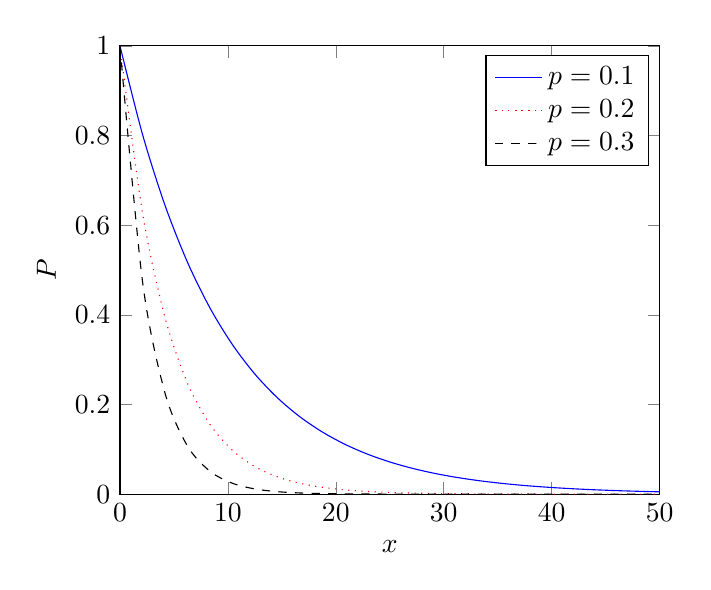
\begin{tikzpicture}
\begin{axis}[
    xlabel={$x$},
	ylabel={$P$},
	yticklabel style={/pgf/number format/fixed,
	    /pgf/number format/precision=1},
	xticklabel style={/pgf/number format/fixed,
	    /pgf/number format/precision=0},
	xmin = 0,
	xmax = 50,
	ymin = 0,
	ymax = 1.0,
	legend entries={$p=0.1$, $p=0.2$, $p=0.3$}
]
\addplot[blue,smooth,solid, domain=0:50] { exp(x*ln(1-0.1) };
\addplot[red,smooth,dotted, domain=0:50] {exp(x*ln(1-0.2))};
\addplot[black,smooth,dashed, domain=0:50] { exp(x*ln(1-0.3) };
\end{axis}
\end{tikzpicture}
}
\bicaption[fig:procheck]{图索引}{成功骗过用户的概率和检测次数的关系}{Fig}{The relation between the possibility of successful cheating and check times}
\end{figure}

我们的基于采样的验证是这样的:在系统的一般使用时为了效率考虑,用户都采用非验证搜索。然后随机的隔一段时间,用户在之前进行的搜索中随机抽出几个,用同样的关键词进行验证搜索。在收到验证搜索的结果后,用户先检验结果证明来保证这次验证搜索是正确的,然后用户在比对这次验证搜索的结果和之前同关键词的非验证搜索的结果。如果两次的结果一致,说明云服务在之前的那次非验证搜索时,没有欺骗用户,结果也是对的。

假设云服务商的搜索不是完全正确的,且错误情况是随机均匀分布的,其错误概率为p。比如说用户先是进行了n次非验证搜索。这时由于没有证明,用户是不知道云服务商给的结果是不是正确的。然后我们在这n次非验证搜索中,随机抽取x个查询来进行采样验证。那么这x个采样都通过,云服务成功骗过用户的概率为:$P = (1-p)^x$。

虽然从这个式子来看,云服务商成功骗过用户的概率和非验证搜索的次数n无关,但是考虑到云服务商可能会分析用户的采样规律,导致采样到云服务出错的情况降低,用户的非验证搜索次数还是要远大于采样数多比较好。

在图\ref{fig:procheck}中,我们列举了在几个不同的错误率上,云服务商成功骗过用户的概率和检测次数的关系。从图中我们可以看出,云服务商成功骗过用户的概率是随采样次数呈指数级降低的。即使云服务上的错误率只有10\%,用户也只要进行50次采样验证就能保证云服务商的错误不被发现的概率基本为0。

\subsection{和客户端验证的区别}
在第\ref{chap:relatedwork}章我们提到过一种客户端验证方式:用户在收到云服务商返回的查询结果后,从里面随机抽出几个查询,然后在本地重新进行搜索。最后通过对比本地搜索的结果和云服务商返回的结果来判断云服务商是否在欺骗用户。

与客户端验证方式类似,我们的基于采样的验证方式也是通过随机抽取一些查询来进行验证,也是只能在一定概率上保证正确性。但和客户端验证不同的是,我们的基于采样的验证方式,不需要用户在本地重新进行搜索,而只需要向云服务商提交一次或多次验证搜索。由于不需要在本地进行搜索,用户不仅节约了很多本地计算时间,还不需要在本地保存文档和索引这些非常占用空间的数据。由于不需要在本地保存文档和索引数据,用户就可以方便地在不同的客户端比如PC、平板或手机上进行查询和采样验证。

我们的采样验证方式之所以比客户端验证方式多了这些优点,是因为我们的系统可以在云服务端生成结果证明。而对于一般的客户端验证方式,云服务端没有这个功能,就只能靠用户在本地重新搜索来验证结果的正确性。

\section{本章小结}
在本章,我们介绍了一种基于RSA Accumulator的验证机制。
整个验证机制可以分为建立可验证的索引、云端检索和验证证明三个步骤。
该验证机制的主要方法是设计了一种可验证索引,然后把文档搜索的过程用集合求交集的方式表示。最后用验证集合求交集的正确性类似的方式来验证搜索结果的正确性。

我们还考虑了一种效率优先而正确性保证可以降低的情况。对于这种情况,我们提出了一种基于采样的验证方式。在这种方式下,用户平时使用的是不需要结果证明的搜索。然后用户在随机的时间,随机选取之前进行过的搜索让云服务商进行带结果证明的搜索。用户可以比较两次搜索的结果来判断云服务商是否有出错的情况。这种基于采样的验证方式使得用户可以在搜索效率和正确性保证度之间进行选择,选择一个适合自己的权衡。
